\chapter{Strømforsyning}
Ud fra kravspecifikation skal delmodulerne (SM og VBTE) kunne drives fra en 24V AC/DC forsynings kilde. Selve modulerne er designet til 12V DC og 5V DC forsyningsspændringer , der designes derfor en strømforsyning der regulere spændingen så den kan levere 12V 1A og 5V 0,5A.  

\section{Overordnet design}
I dette afsnit beskrives og vises det overordnede hardware blokdiagram over strømforsyningen samt beskrivelse signaler.

\begin{figure}[H]
\centering
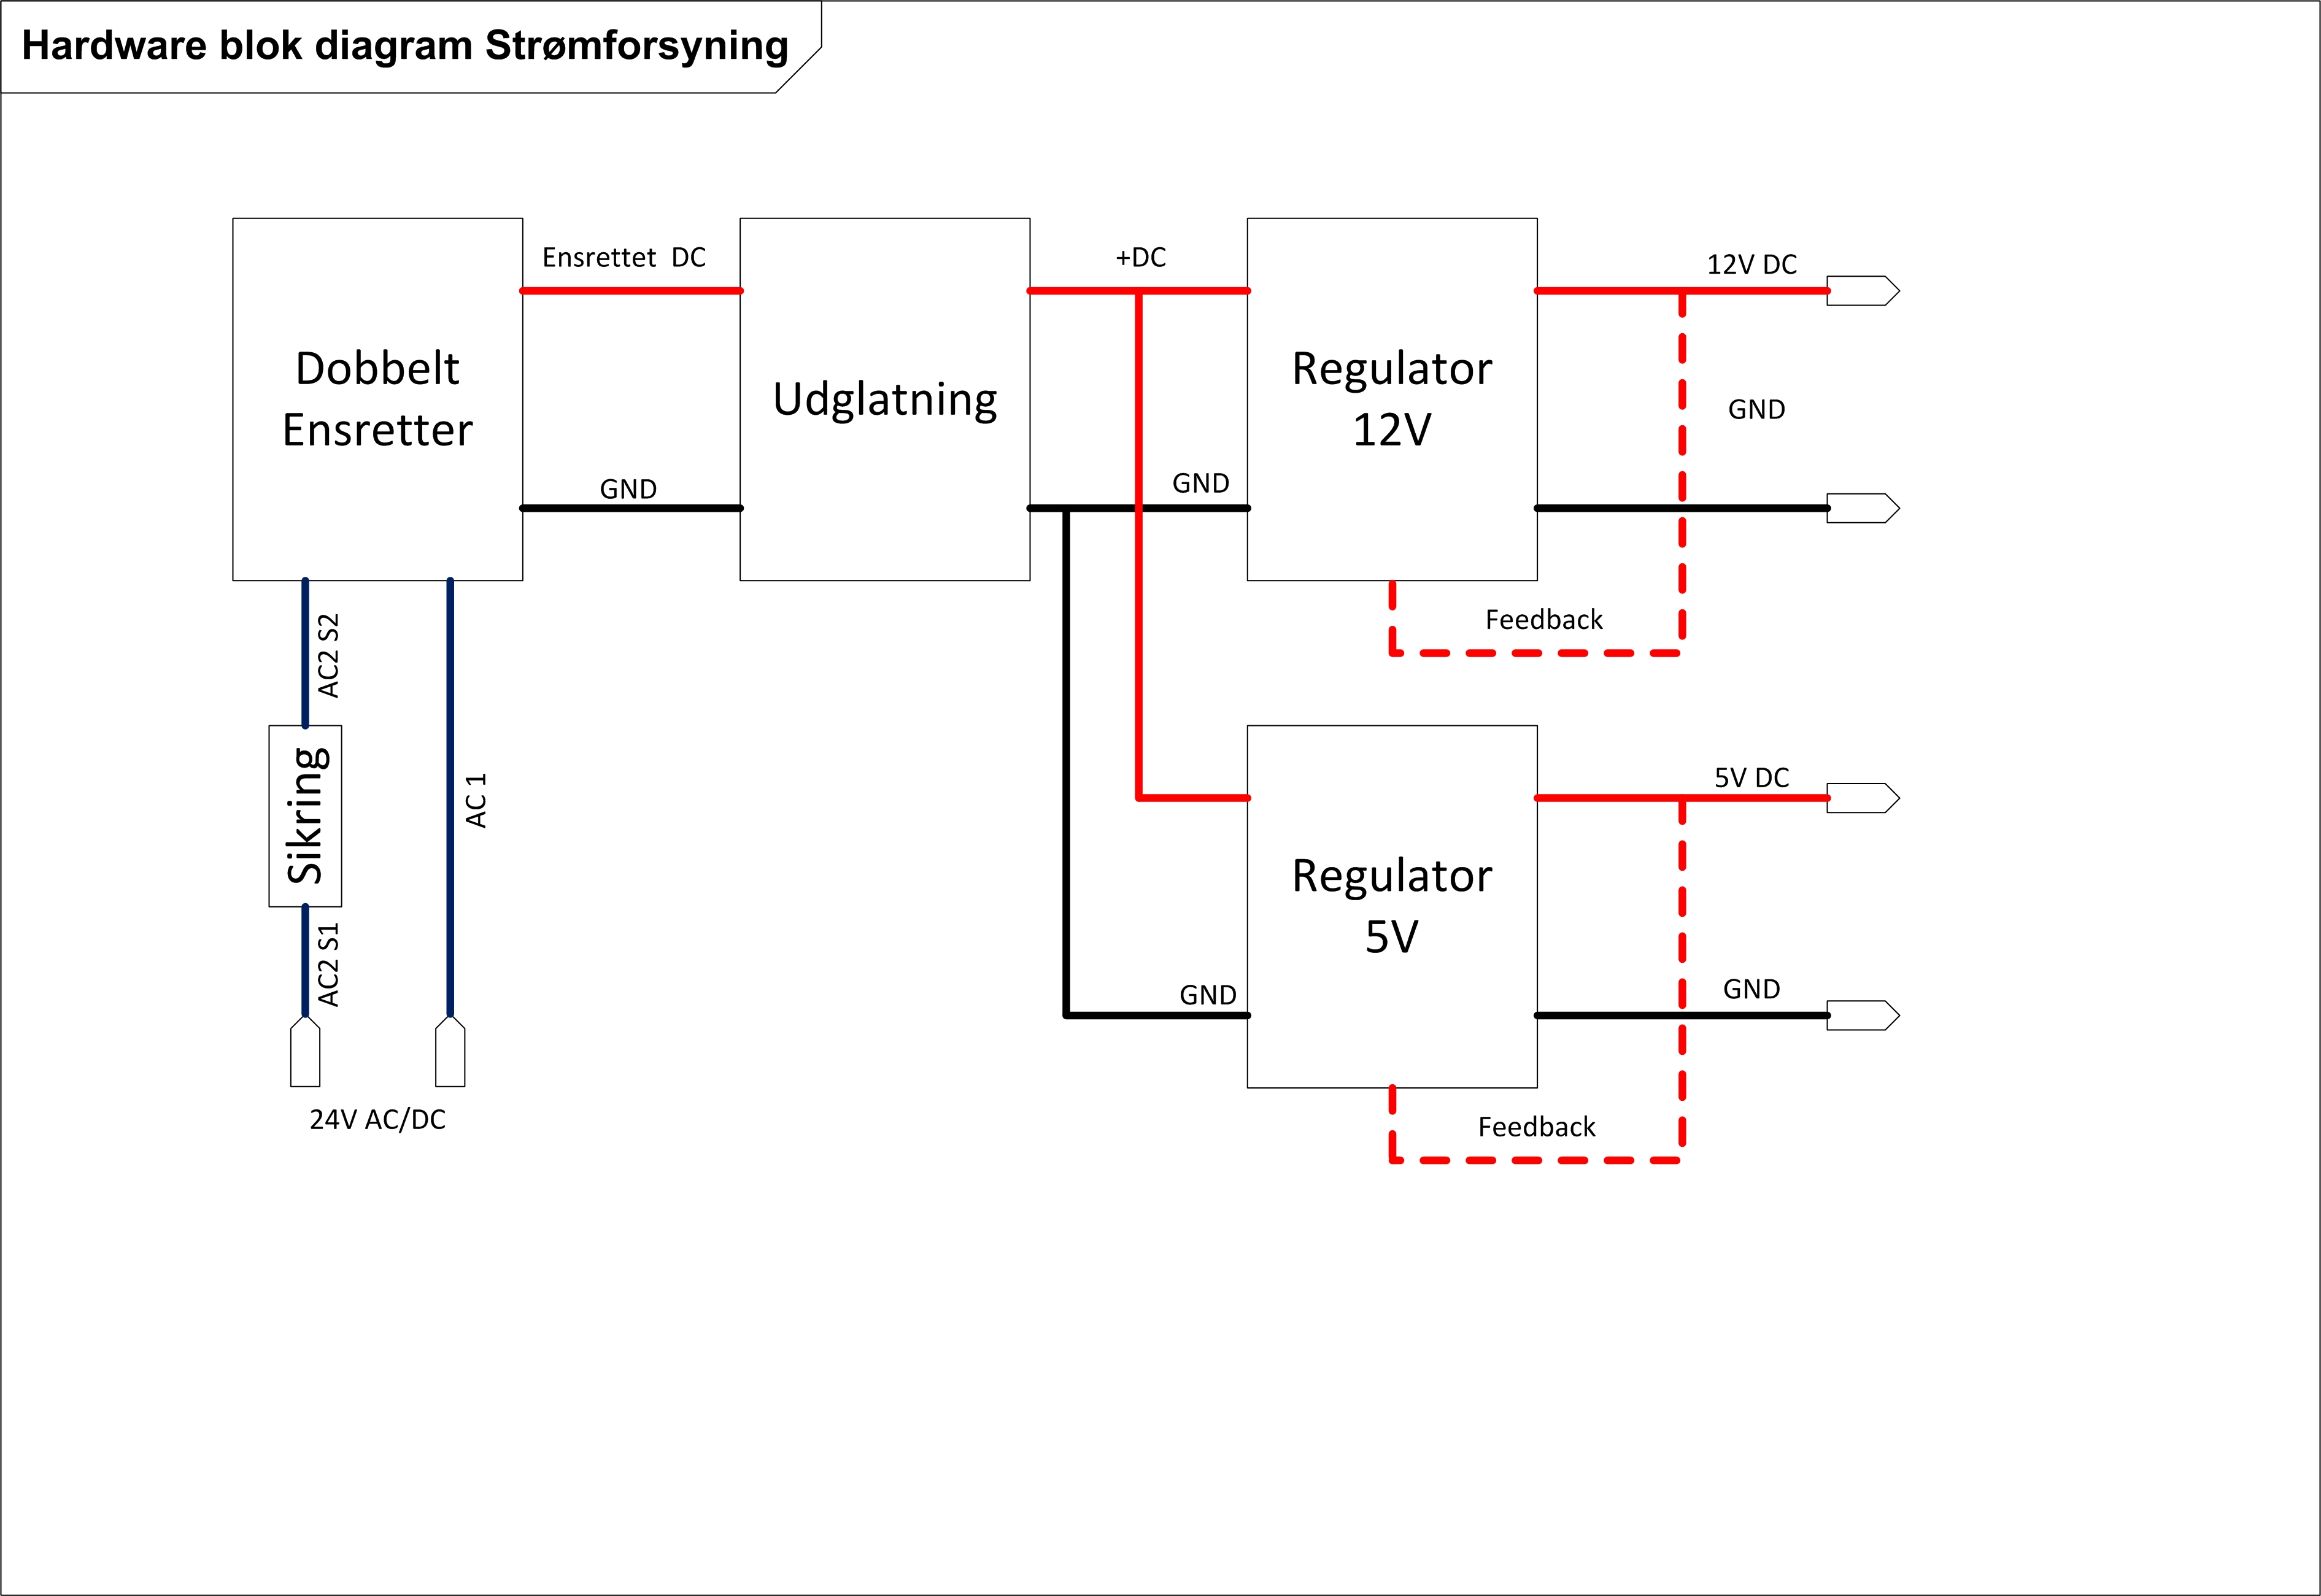
\includegraphics[width=1\textwidth]{billeder/PowerSupplyBlok}
\caption{Overordnet blokdiagram for strømforsyning}
\label{fig:PowerSubbly Blok}
\end{figure}